\begin{frame}[fragile]{Comandos básicos - Iniciar un repositorio}
  \begin{columns}[onlytextwidth]
    \column{0.6\textwidth}
    \alert{Inicializar un repositorio}
    \begin{minted}{console}
    $ git init
    \end{minted}

    \alert{Clonar un repositorio de un remoto (\faGithubAlt GitHub!)}
    \begin{minted}{console}
    $ git clone <url>
    \end{minted}
    \column{0.4\textwidth}
    \tikzstyle{every node}=[draw=solarized-base1,thick,anchor=west]
    \tikzstyle{selected}=[draw=solarized-green,fill=solarized-green!30]
    \begin{tikzpicture}[%
      grow via three points={one child at (0.5,-0.7) and
      two children at (0.5,-0.7) and (0.5,-1.4)},
      edge from parent path={(\tikzparentnode.south) |- (\tikzchildnode.west)}]
      \node {repository}
        child { node [selected] {.git}}
        child { node {source}}
        child { node {LICENSE}}
        child { node {README.md}};
    \end{tikzpicture}
  \end{columns}
\end{frame}

\begin{frame}[fragile]{Comandos básicos - Preparar y confirmar}
  \alert{Añadir un archivo al área de preparación}
  \begin{minted}{console}
    $ git add <archivo>
  \end{minted}

  \alert{Confirmar los cambios}
  \begin{minted}{console}
    $ git commit
    $ git commit -m 'mensaje'
  \end{minted}

  \alert{Saltarse el área de preparación}
  \begin{columns}[onlytextwidth]
  \column{0.6\textwidth}
  \begin{minted}{console}
    $ git commit -a -m 'mensaje'
  \end{minted}
  \column{0.4\textwidth}
    Sólo prepara y confirma los archivos que Git está rastreando!
  \end{columns}

  \begin{tikzpicture}[remember picture,overlay]
    \node[anchor=north east, inner xsep=45pt, inner ysep=60pt] at (current page.north east) {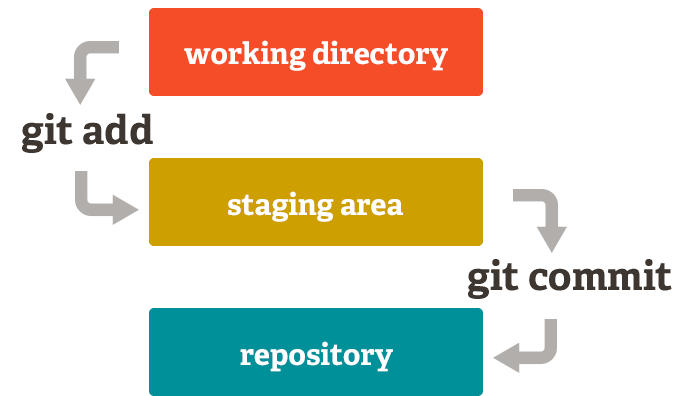
\includegraphics[scale=0.2]{images/areas}};
  \end{tikzpicture}
\end{frame}

\begin{frame}[fragile]{Comandos básicos - Revisar el estado}
  \begin{columns}[onlytextwidth]
  \column{0.35\textwidth}
  Diferencia entre archivos preparados, no preparados pero rastreados y no rastreados.
  \begin{minted}{console}
    $ git status
    $ git status -s
  \end{minted}
  \column{0.02\textwidth}
  \column{0.63\textwidth}
  \vspace{0.3cm}
  \begin{minted}[escapeinside=||, frame=single, framerule=1pt, fontsize=\scriptsize, bgcolor=solarized-base1!30]{console}
[user@linux ~]$ git status
On branch master
Changes to be committed:
(use "git reset HEAD <file>..." to unstage)
|  {\color{solarized-green}new file:   presentation.tex}|
|  {\color{solarized-green}deleted:    basura.text}|
Changes not staged for commit:
(use "git add <file>..." to update what will be committed)
(use "git checkout -- <file>..." to discard changes in working directory)
|  {\color{solarized-red}modified:   .gitignore}|
Untracked files:
(use "git add <file>..." to include in what will be committed)
|  {\color{solarized-red}configuration.tex}|
  \end{minted}
  \end{columns}
\end{frame}

\begin{frame}[fragile]{Comandos básicos - Revisar el estado}
  \begin{columns}[onlytextwidth]
  \column{0.35\textwidth}
  \begin{tabular}{rcl}
    \texttt{A} & $\Rightarrow$ & Nuevo \\
    \texttt{M} & $\Rightarrow$ & Modificado \\
    \texttt{D} & $\Rightarrow$ & Eliminado \\
    \texttt{?} & $\Rightarrow$ & No rastreado \\
  \end{tabular}
  \column{0.02\textwidth}
  \column{0.63\textwidth}
  \begin{minted}[escapeinside=||, frame=single, framerule=1pt, fontsize=\scriptsize, bgcolor=solarized-base1!30]{console}
[user@linux ~]$ git status -s
| {\color{solarized-red}M}| .gitignore
|{\color{solarized-green}D} | basura.text
|{\color{solarized-green}A} | presentation.tex
|{\color{solarized-red}??}| configuration.tex
  \end{minted}
  \begin{center}
  $1^a$ columna: En estado preparado \\
  $2^a$ columna: En estado no preparado
  \end{center}
  \end{columns}
\end{frame}

\begin{frame}[fragile]{Comandos básicos - Eliminar y Renombrar}
  \alert{Eliminar}
  \begin{itemize}
    \item Eliminar un archivo no preparado y preparar la eliminación
    \begin{minted}{console}
  $ git rm <archivo>
    \end{minted}
    \item Eliminar un archivo preparado y preparar la eliminación
    \begin{minted}{console}
  $ git rm -f <archivo>
    \end{minted}
    \item Dejar de rastrear sin eliminar
    \begin{minted}{console}
  $ git rm --cached <archivo>
    \end{minted}
  \end{itemize}

  \alert{Renombrar}
  \begin{minted}{console}
    $ git mv <archivo> <archivo-nuevo>
  \end{minted}

\end{frame}
